\documentclass[12pt]{article}
\usepackage{amsmath}
\usepackage{amssymb}
\usepackage{amsthm}
\usepackage{amsfonts}
\usepackage{graphicx}
\usepackage{textcomp}
\usepackage{hyperref}
\usepackage{tikz}
\usepackage{enumitem}
\usepackage{mathtools}
\usepackage{enumitem}
\usepackage{wasysym}
\usepackage{ulem}
\usepackage{xspace}
\usepackage{csquotes}
\usepackage{booktabs}

\DeclareMathOperator{\dist}{dist}
\DeclareMathOperator{\Nul}{Nul}
\DeclareMathOperator{\Row}{Row}
\DeclareMathOperator{\proj}{proj}

\setlength{\arraycolsep}{12pt}

\newcommand{\defn}{\textbf{Def.}\xspace}
\newcommand{\thm}{\textbf{Thm.}\xspace}
\newcommand{\ex}{\textbf{ex.}\xspace}
\newcommand{\Ex}{\textbf{Ex.}\xspace}
\newcommand{\ie}{\textbf{i.e.}\xspace}
\newcommand{\lemma}{\textit{Lemma}\xspace}
\newcommand{\bproof}{\textit{Proof ($\impliedby$).}\xspace}
\newcommand{\fproof}{\textit{Proof ($\implies$).}\xspace}
\newcommand{\bigEps}{\mathcal{E}}
\newcommand{\soln}{\textit{Soln.}\xspace}

\renewcommand{\arraystretch}{1.25} % Adjust row spacing


\hypersetup{
    colorlinks=true,
    linkcolor=blue,
    filecolor=blue,      
    urlcolor=blue,
}

\newcommand{\ulhref}[2]{\href{#1}{\color{blue}\uline{#2}}}

\begin{document}

\title{MACM 316 Lecture 21}
\author{Alexander Ng}
\date{Friday, February 28, 2025}

\maketitle

\section{Continued from Lecture 20}

Our next task is to develop estimates for the error. As it turns out, the form
of the error (but not necessarily the magnitude) resembles that of the $n^{th}$
Taylor Polynomial.

\subsection{Error Estimates}

\thm (3.3 of Text)

Suppose $x_0, \dots, x_n$ are distinct numbers in the interval $[a,b]$ and
$f\in C^{n+1}[a,b]$. Then for each $x\in [a,b]$, a number $\xi(x)\in(a,b)$
exists with the property

\[
  f(x) = P(x) + \frac{f^{(n+1)}(\xi(x))}{(n+1)!} (x-x_0) (x-x_1) \dots (x-x_n)
.\]

\begin{center}

\begin{tikzpicture}[overlay, remember picture]
    \draw[thick,->] (-2,0) node[below]{\textbf{n-th Langrange Interpolating Polynomial}} to (-3.2,0.6);
\end{tikzpicture}
\end{center}

Recall: If $f$ has $(n+1)$ continuous derivatives on $[a,b]$ and $P(x)$ is the 
interpolating polynomial of degree $\leq n$ for $f$ at the points 
$x_0, \dots, x_n$, then,

\[
  f(x) - P(x) = \frac{f^{(n+1)}(\xi (x))}{(n+1)!} \prod_{k=0}^{n} (x-x_k)
.\]

\Ex suppose you need to construct six-decimal-place tables for the common, or
base-10, logarithm function from $x=1$ to $x=10$ in a way that linear 
interpolation is accurate within $10^{-6}$ of the true value. Determine a bound
for the step size for this table.

Based on the following data:

\begin{table}[h]
    \centering
    \begin{tabular}{c c c}
        \toprule
        $i$ & $x_i$ & $f(x_i)$ \\
        \midrule
        0 & 3.2 & 22.0 \\
        1 & 2.7 & 17.8 \\
        2 & 1.0 & 14.2 \\
        3 & 4.8 & 38.3 \\
        4 & 5.6 & 51.7 \\
        \bottomrule
    \end{tabular}
    % \caption{Tabulated data of $x_i$ and $f(x_i)$ values}
    % \label{tab:data}
\end{table}

find approximations to $f(3)$ using the $2^{nd}$ and $3^{rd}$ Lagrange
interpolating polynomials.

\soln we will use $x_0, x_1$ and $x_3$ to build the $2^{nd}$ Lagrange
interpreting polynomial.

\begin{align*}
P_2(3) &= \frac{(3 - 2.7)(3 - 4.8)}{(3.2 - 2.7)(3.2 - 4.8)} (22.0) \\
&\quad + \frac{(3 - 3.2)(3 - 4.8)}{(2.7 - 3.2)(2.7 - 4.8)} (17.8) \\
&\quad + \frac{(3 - 3.2)(3 - 2.7)}{(4.8 - 3.2)(4.8 - 2.7)} (38.3) \\
&\approx 20.27
\end{align*}

We will use $x_0, x_1, x_2, x_3$ to build the $3^{rd}$ Lagrange
interpolating polynomial.

\begin{align*}
P_3(3) &= \frac{(3.0 - 2.7)(3.0 - 1.0)(3.0 - 4.8)}{(3.2 - 2.7)(3.2 - 1.0)(3.2 - 4.8)} (22.0) \\
&\quad + \frac{(3.0 - 3.2)(3.0 - 1.0)(3.0 - 4.8)}{(2.7 - 3.2)(2.7 - 1.0)(2.7 - 4.8)} (17.8) \\
&\quad + \frac{(3.0 - 3.2)(3.0 - 2.7)(3.0 - 4.8)}{(1.0 - 3.2)(1.0 - 2.7)(1.0 - 4.8)} (14.2) \\
&\quad + \frac{(3.0 - 3.2)(3.0 - 2.7)(3.0 - 1.0)}{(4.8 - 3.2)(4.8 - 2.7)(4.8 - 1.0)} (38.3) \\
&\approx 20.21
\end{align*}

Notice that:

\begin{enumerate}
\item We do not know the derivative values of $f$, therefore we cannot apply 
  the error formula. However, we can make an estimate for the error by examining
  polynomials of different degrees by using different nodes.

\item The $P_2$-calculation was not used to reduce the work in calculating $P_3$.
  We want to find a way to use previous degrees of $P$, especially since the 
  previous point implies that we will examine the results for Lagrange 
  polynomials of varying degrees.
\end{enumerate}

\noindent
We want to examine polynomials based on different nodes. In the last example, 
we considered the polynomial based on the nodes $x_0, x_1 \text{ and } x_3$

We will call this polyomial $\mathbf{P_{013}(x)}$

\noindent
We also considered the polynomial based on the nodes $x_0, x_1, x_2, x_3$

We will call this polyomial $\mathbf{P_{0123}(x)}$

Similarly, we make the following definition:

Let $f$ be a function defined at $x_0, x_1, x_2, \dots, x_n$ and suppose that
$m_1, m_2, \dots ,m_k$ are $k$ distinct integers with $0\leq m_i \leq n$ and
for each $i$. 

The Lagrange Interpolating Polynomial that agrees with $f$ at 
$x_m, x_{m2}, \dots, x_{mk}$ is denoted

\[
  P_{m_1, m_2, \dots, m_k}
.\]

Using this notation,

\[
P_0(x) = f(x_0)
\]

\[
P_1(x) = \frac{(x - x_1) f(x_0) + (x - x_0) f(x_1)}{x_0 - x_1}
\]

and 


\begin{align*}
  P_{0,1}(x) &= \left( \frac{x - x_1}{x_0 - x_1} \right) f(x_0) + \left( \frac{x - x_0}{x_1 - x_0} \right) f(x_1) \\
             &= \frac{(x - x_1) P_0(x) - (x - x_0) P_1(x)}{x_0 - x_1}
\end{align*}

So $P_{0,1}(x)$ can be recursively defined in terms of $P_0(x)$ and $P_1(x)$.

More generally:

\thm Let $f$ be defined at $x_0, x_1, \dots, x_k$ and $x_j$ and $x_i$ be two
distinct numbers in this set. Then

\[
  P_{0,1,\dots,k}(x) = 
  \frac{(x - x_j) P_{0,1,\dots,j,j+1,\dots,n}(x) - (x - x_i) P_{0,1,\dots,i-1,i+1,\dots,n}(x)}{x_i - x_j}
.\]

\proof I left out the proof.

The corresponding procedure is called Neville's Method. Here, values for each 
interpolating polynomial are generated using previous calculations.

\Ex $\displaystyle P_{0,1}(x) = \frac{(x-x_1)P_0 - (x-x_0) P_1}{(x_0 - x_1)}$ is
derived from $P_0 + P_1$. Correspondingly, $P_{1,2}(x)$ is derived from $P_1$
and $P_2$.

Written as a table:

\begin{figure}[h]
    \centering
    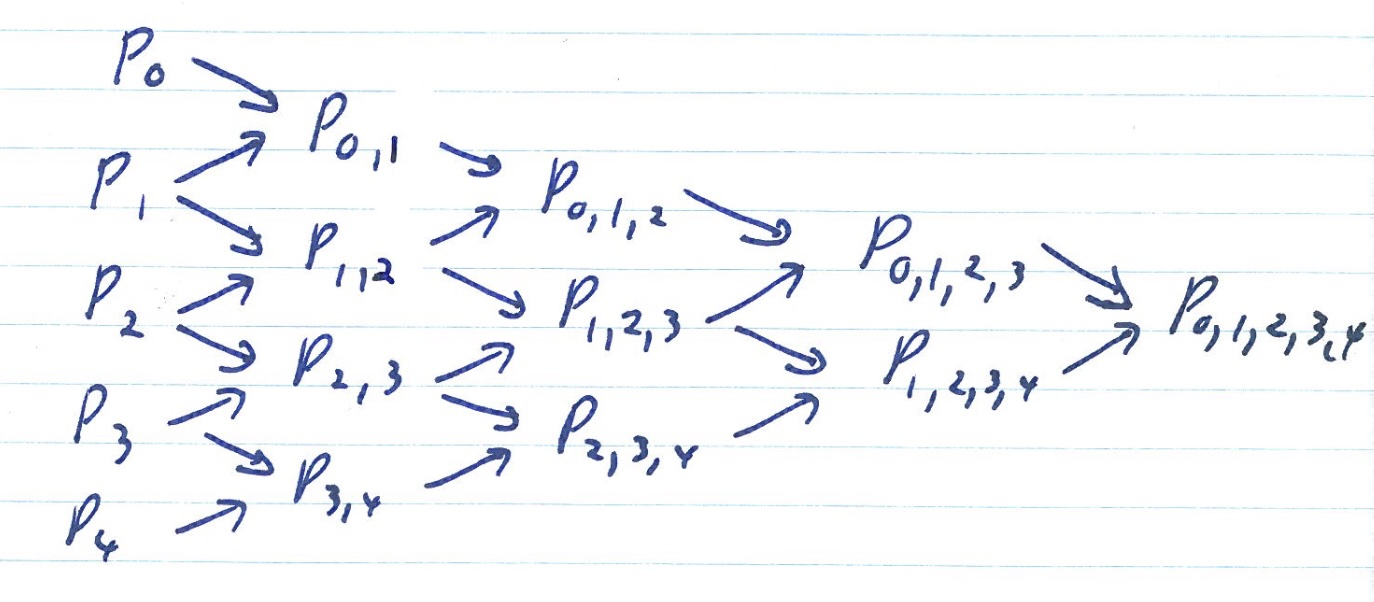
\includegraphics[width=0.8\textwidth]{Lecture 021 Neville's Method Table.jpg}
\end{figure}

\Ex suppose $x_j = j$ for $j=0,1,2,3$ and it is known that 

\begin{align*}
  &P_{0,1}(x) = 2x+1 \\
  &P_{0,2}(x) = x+1 \\
  &P_{1,2,3}(2.5) = 3
\end{align*}

Find $P_{0123}(2.5)$.

We have $P_{123}$ and we need another quadratic to find our $P_{0123}$

\[
P_{0,1,2} = \frac{(x-x_1)P_{02} (x) - (x-x_2) P_{01}(x)}{x_2 - x_1}
.\]

We evaluate $P_{02}(2.5) = 2.25$ and $P_{01}(2.5) = 6$

We have $x_1 = 1, x_2 = 2, x=2.5$

\[
  P_{012}(2.5) = 2.25 
.\]

\[
  P_{0123}(2.5) = \frac{(2.25-x_0)P_{123}(2.25) - (2.25-x_3)P_{012}(2.25)}{x_3 -
  x_0} = 2.875
\]

\end{document}
